\documentclass{article}

  % packages
    % basic stuff for rendering math
    \usepackage[letterpaper, top=1in, bottom=1in, left=1in, right=1in]{geometry}
    \usepackage[utf8]{inputenc}
    \usepackage[english]{babel}
    \usepackage{amsmath} 
    \usepackage{amssymb}

    % extra math symbols and utilities
    \usepackage{mathtools}        % for extra stuff like \coloneqq
    \usepackage{mathrsfs}         % for extra stuff like \mathsrc{}
    \usepackage{centernot}        % for the centernot arrow 
    \usepackage{bm}               % for better boldsymbol/mathbf 
    \usepackage{enumitem}         % better control over enumerate, itemize
    \usepackage{hyperref}         % for hypertext linking
    \usepackage{xr-hyper}
    \usepackage{fancyvrb}          % for better verbatim environments
    \usepackage{newverbs}         % for texttt{}
    \usepackage{xcolor}           % for colored text 
    \usepackage{listings}         % to include code
    \usepackage{lstautogobble}    % helper package for code
    \usepackage{parcolumns}       % for side by side columns for two column code
    

    % page layout
    \usepackage{fancyhdr}         % for headers and footers 
    \usepackage{lastpage}         % to include last page number in footer 
    \usepackage{parskip}          % for no indentation and space between paragraphs    
    \usepackage[T1]{fontenc}      % to include \textbackslash
    \usepackage{footnote}
    \usepackage{etoolbox}

    % for custom environments
    \usepackage{tcolorbox}        % for better colored boxes in custom environments
    \tcbuselibrary{breakable}     % to allow tcolorboxes to break across pages

    % figures
    \usepackage{pgfplots}
    \pgfplotsset{compat=1.18}
    \usepackage{float}            % for [H] figure placement
    \usepackage{tikz}
    \usepackage{tikz-cd}
    \usepackage{circuitikz}
    \usetikzlibrary{arrows}
    \usetikzlibrary{positioning}
    \usetikzlibrary{calc}
    \usepackage{graphicx}
    \usepackage{algorithmic}
    \usepackage{caption} 
    \usepackage{subcaption}
    \captionsetup{font=small}

    % for tabular stuff 
    \usepackage{dcolumn}

    \usepackage[nottoc]{tocbibind}
    \pdfsuppresswarningpagegroup=1
    \hfuzz=5.002pt                % ignore overfull hbox badness warnings below this limit

  % New and replaced operators
    \DeclareMathOperator{\Tr}{Tr}
    \DeclareMathOperator{\Sym}{Sym}
    \DeclareMathOperator{\Span}{span}
    \DeclareMathOperator{\std}{std}
    \DeclareMathOperator{\Cov}{Cov}
    \DeclareMathOperator{\Var}{Var}
    \DeclareMathOperator{\Corr}{Corr}
    \DeclareMathOperator{\pos}{pos}
    \DeclareMathOperator*{\argmin}{\arg\!\min}
    \DeclareMathOperator*{\argmax}{\arg\!\max}
    \newcommand{\ket}[1]{\ensuremath{\left|#1\right\rangle}}
    \newcommand{\bra}[1]{\ensuremath{\left\langle#1\right|}}
    \newcommand{\braket}[2]{\langle #1 | #2 \rangle}
    \newcommand{\qed}{\hfill$\blacksquare$}     % I like QED squares to be black

  % Custom Environments
    \newtcolorbox[auto counter, number within=section]{question}[1][]
    {
      colframe = orange!25,
      colback  = orange!10,
      coltitle = orange!20!black,  
      breakable, 
      title = \textbf{Question \thetcbcounter ~(#1)}
    }

    \newtcolorbox[auto counter, number within=section]{exercise}[1][]
    {
      colframe = teal!25,
      colback  = teal!10,
      coltitle = teal!20!black,  
      breakable, 
      title = \textbf{Exercise \thetcbcounter ~(#1)}
    }
    \newtcolorbox[auto counter, number within=section]{solution}[1][]
    {
      colframe = violet!25,
      colback  = violet!10,
      coltitle = violet!20!black,  
      breakable, 
      title = \textbf{Solution \thetcbcounter}
    }
    \newtcolorbox[auto counter, number within=section]{lemma}[1][]
    {
      colframe = red!25,
      colback  = red!10,
      coltitle = red!20!black,  
      breakable, 
      title = \textbf{Lemma \thetcbcounter ~(#1)}
    }
    \newtcolorbox[auto counter, number within=section]{theorem}[1][]
    {
      colframe = red!25,
      colback  = red!10,
      coltitle = red!20!black,  
      breakable, 
      title = \textbf{Theorem \thetcbcounter ~(#1)}
    } 
    \newtcolorbox[auto counter, number within=section]{proposition}[1][]
    {
      colframe = red!25,
      colback  = red!10,
      coltitle = red!20!black,  
      breakable, 
      title = \textbf{Proposition \thetcbcounter ~(#1)}
    } 
    \newtcolorbox[auto counter, number within=section]{corollary}[1][]
    {
      colframe = red!25,
      colback  = red!10,
      coltitle = red!20!black,  
      breakable, 
      title = \textbf{Corollary \thetcbcounter ~(#1)}
    } 
    \newtcolorbox[auto counter, number within=section]{proof}[1][]
    {
      colframe = orange!25,
      colback  = orange!10,
      coltitle = orange!20!black,  
      breakable, 
      title = \textbf{Proof. }
    } 
    \newtcolorbox[auto counter, number within=section]{definition}[1][]
    {
      colframe = yellow!25,
      colback  = yellow!10,
      coltitle = yellow!20!black,  
      breakable, 
      title = \textbf{Definition \thetcbcounter ~(#1)}
    } 
    \newtcolorbox[auto counter, number within=section]{example}[1][]
    {
      colframe = blue!25,
      colback  = blue!10,
      coltitle = blue!20!black,  
      breakable, 
      title = \textbf{Example \thetcbcounter ~(#1)}
    } 
    \newtcolorbox[auto counter, number within=section]{code}[1][]
    {
      colframe = green!25,
      colback  = green!10,
      coltitle = green!20!black,  
      breakable, 
      title = \textbf{Code \thetcbcounter ~(#1)}
    } 
    \newtcolorbox[auto counter, number within=section]{algo}[1][]
    {
      colframe = green!25,
      colback  = green!10,
      coltitle = green!20!black,  
      breakable, 
      title = \textbf{Algorithm \thetcbcounter ~(#1)}
    } 

    \definecolor{dkgreen}{rgb}{0,0.6,0}
    \definecolor{gray}{rgb}{0.5,0.5,0.5}
    \definecolor{mauve}{rgb}{0.58,0,0.82}
    \definecolor{darkblue}{rgb}{0,0,139}
    \definecolor{lightgray}{gray}{0.93}
    \renewcommand{\algorithmiccomment}[1]{\hfill$\triangleright$\textcolor{blue}{#1}}

    % default options for listings (for code)
    \lstset{
      autogobble,
      frame=ltbr,
      language=Python,
      aboveskip=3mm,
      belowskip=3mm,
      showstringspaces=false,
      columns=fullflexible,
      keepspaces=true,
      basicstyle={\small\ttfamily},
      numbers=left,
      firstnumber=1,                        % start line number at 1
      numberstyle=\tiny\color{gray},
      keywordstyle=\color{blue},
      commentstyle=\color{dkgreen},
      stringstyle=\color{mauve},
      backgroundcolor=\color{lightgray}, 
      breaklines=true,                      % break lines
      breakatwhitespace=true,
      tabsize=3, 
      xleftmargin=2em, 
      framexleftmargin=1.5em, 
      stepnumber=1
    }

  % Page style
    \pagestyle{fancy}
    \fancyhead[L]{Linear Classification}
    \fancyhead[C]{Muchang Bahng}
    \fancyhead[R]{Spring 2025} 
    \fancyfoot[C]{\thepage / \pageref{LastPage}}
    \renewcommand{\footrulewidth}{0.4pt}          % the footer line should be 0.4pt wide
    \renewcommand{\thispagestyle}[1]{}  % needed to include headers in title page

  % external documents 
  %  \externaldocument[place-]{../Machine_Learning/paper}[../Machine_Learning/paper.pdf] 

\begin{document}

\title{Linear Classification}
\author{Muchang Bahng}
\date{Spring 2025}

\maketitle
\tableofcontents
\pagebreak

This covers computability theory, complexity theory, and automata theory. 
Alphabet. Boolean logic


\section{Perceptron} 

  The perceptron uses a linear regression function as a plugin-classifier, inspired by the artificial modeling of a human neuron \cite{1943mcculloch}. 

  \begin{definition}[Perceptron]
    The \textbf{perceptron model} is a discriminative linear classifier that assigns 
    \begin{equation}
      f_w (x) = \begin{cases} 1 & \text{ if } w^T x + b \geq 0 \\ -1 & \text { if } w^T x + b < 0 \end{cases}
    \end{equation}
    where we have chosen to label class $C_1 = 1$ and $C_2 = -1$. 
  \end{definition}

  Note that unlike linear regression (and logistic regression, as we will see later), the perceptron is not a probabilistic model. It is a \textit{discriminant function}, which just gives point estimates of the classes, not their respective probabilities. Like logistic regression, however, it is a linear model, meaning that the decision boundary it creates is always a linear (affine) hyperplane. 

  To construct the surrogate loss function, we would want a loss that penalizes not only if there is a misclassification, but how \textit{far} that misclassified point is from the boundary. Therefore, if $y$ and $\hat{y} = f_w (x)$ have the same sign, i.e. if $y f_w (x) > 0$, then the penalty should be $0$, and if it is $< 0$, then the penalty should be proportional to the orthogonal distance of the misclassified point to the boundary, which is represented by $-wT x y$ (where the negative sign makes this cost term positive). 

  \begin{definition}[Surrogate Loss for Perceptron]
    Therefore, our cost functions would take all the points and penalize all the terms by $0$ if they are correctly classified and by $-\mathbf{w}^T \boldsymbol{\phi}^{(n)} y^{(n)}$ if incorrectly classified. 
    \begin{equation}
      L(y, \hat{y}) = \sum_{n=1} [ -\mathbf{w}^T \boldsymbol{\phi}^{(n)} y^{(n)} ]_+ \text{ where } [f(\mathbf{x})]_+ \coloneqq \begin{cases} f(\mathbf{x}) & \text{ if } f(\mathbf{x}) > 0 \\ 0 & \text{ else } \end{cases}
    \end{equation}
    Note that this is a piecewise linear function and convex. 
  \end{definition}

  \begin{code}[Perceptron in scikit-learn]
    Let's implement this in scikit-learn, using two pipelines with different data standardization techniques to see the differences in the perceptron boundary. 

    \begin{figure}[H]
      \centering 
      \begin{lstlisting}
        from sklearn.pipeline import Pipeline 
        from sklearn.linear_model import Perceptron
        from sklearn.preprocessing import QuantileTransformer, StandardScaler

        pipe1 = Pipeline([ 
            ("scale", StandardScaler()), 
            ("model", Perceptron())
        ])

        pipe2 = Pipeline([
            ("scale", QuantileTransformer(n_quantiles=100)), 
            ("model", Perceptron())
        ])
      \end{lstlisting}
      \caption{} 
    \end{figure}

    \begin{figure}[H]
      \centering
      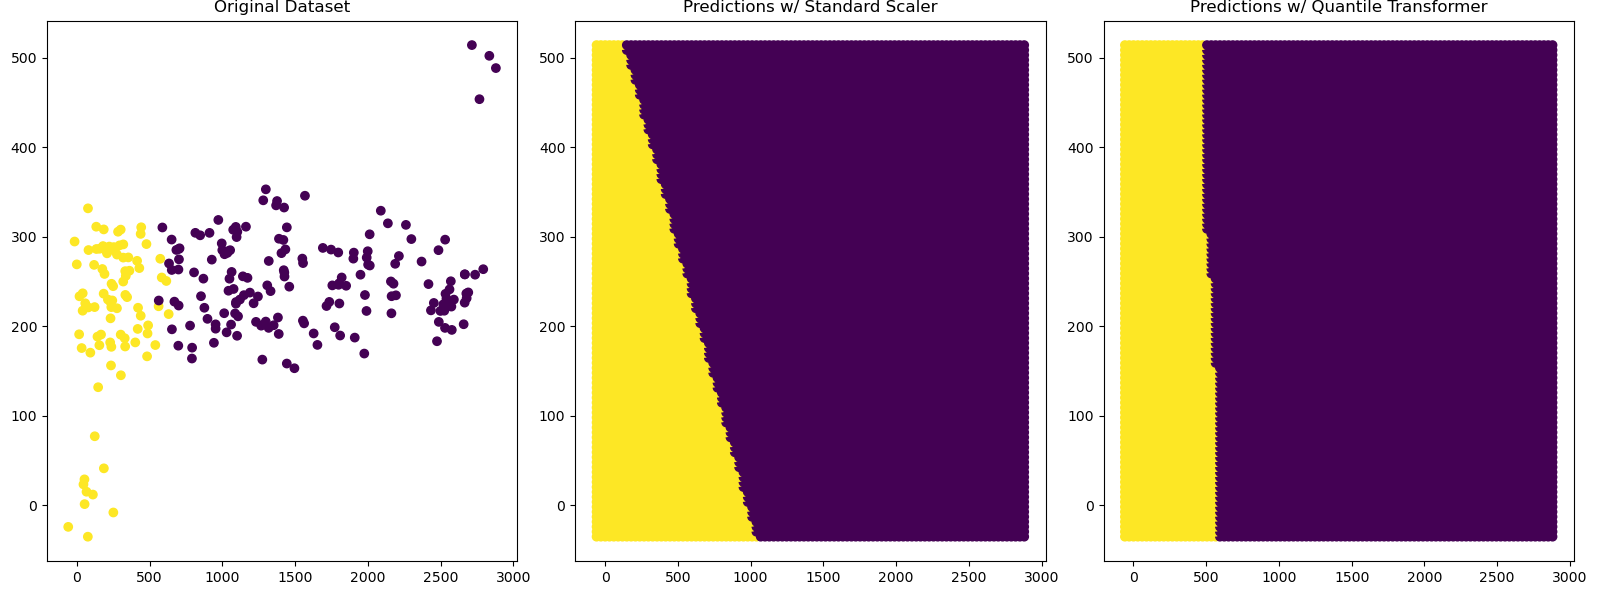
\includegraphics[scale=0.35]{img/Perceptron.png}
      \caption{Perceptron Trained on Different Standardized Data}
    \end{figure}
  \end{code}


\section{Logistic Regression} 

  We can upgrade from a discriminant function to a discriminative probabilistic model with \textbf{logistic regression}. In linear regression, we assumed that the targets are linearly dependent with the covariates as $y = w^T x + b$. However, this means that the hypothesis $f_w$ is unbounded. Since we have two classes (say with labels $0$ and $1$), we must have some sort of \textit{link function} $\sigma$ that takes the real numbers and compresses it into the domain $[0, 1]$. Technically, we can choose any continuous, monotinically increasing function from $\mathbb{R}$ to $(0, 1)$. However, the following property of the \textit{sigmoid function} $\sigma(x) \coloneqq \frac{1}{1 + e^{x}}$ makes derivation of gradients very nice. \begin{equation}
    \sigma^\prime (x) = \sigma(x) \, \big(1 - \sigma(x) \big)
  \end{equation}

  \begin{definition}[Logistic Regression]
    The \textbf{logistic regression} model is probabilistic discriminative classification model  
    \begin{equation}
      Y \mid X = x \sim \mathrm{Bernoulli}(f(x)), \qquad f(x) = \sigma(\beta^T x)
    \end{equation}
    where $\sigma$ is the sigmoid function. It has parameters $\beta$. 
  \end{definition} 

  One important observation to make is that notice that the output of our hypothesis is used as a parameter to define our residual distribution. 
  \begin{enumerate}
    \item In linear regression, the $f$ was used as the \textit{mean} $\mu$ of a Gaussian. 
    \item In logistic regression, the $f$ is used also as the mean $p$ of a Bernoulli. 
  \end{enumerate}
  The reason we want this sigmoid is so that we make the domains of the means of the residuals match the range of the outputs of our model. It's simply a manner of convenience, and in fact we could have really chose any function that maps $\mathbb{R}$ to $(0, 1)$.\footnote{Some questions may arise, such as ``why isn't the variance parameter of the Gaussian considered in the linear model?" or ``what about other residual distributions that have multiple parameters?" This is all answered by generalized linear models, which uses the output of a linear model as a \textit{natural parameter} of the canonical exponential family of residual distributions. }

  Note that logistic regression has a \textit{nonlinear regression function}, but a \textit{linear decision boundary}. That is, by running this model through the plugin classifier, this becomes a linear classifier. 

  \begin{theorem}[Decision Boundary is Linear]
    The decision boundary of logistic regression is linear. 
  \end{theorem}
  \begin{proof}
    We can solve 
    \begin{equation}
      \frac{1}{1 + e^{\beta^T x}} = \frac{1}{2} \implies 2 = 1 + e^{\beta^T x} \implies 1 = e^{\beta^T x} \implies 0 = \beta^T x
    \end{equation}
    which defines a linear hyperplane orthogonal to vector $\beta$. 
  \end{proof} 

\subsection{Maximum Likelihood Estimation} 

  Our next job is to define a loss to optimize. The pdf of a Bernoulli is not well-defined, but we can smoothly interpolate between the two points at $x = 0$ and $x = 1$ to get a smooth surrogate likelihood.  

  \begin{lemma}[Likelihood for Bernoulli]
    A surrogate likelihood of a $\mathrm{Bernoulli}(p)$ random variable is 
    \begin{equation}
      \mathbb{P}(X = x) = p^x (1 - p)^{1 - x}
    \end{equation} 
    TBD. Why do we express it in this form? Just for convenience? 
  \end{lemma} 
  \begin{proof}
    Just substitute $\mathbb{P}(X = 1) = p^1 (1 - p)^{0} = p$ and $\mathbb{P}(X = 0) = p^0 (1 - p)^1 = 1 - p$. 
  \end{proof}

  Therefore, by taking the negative log-likelihood, we can get our loss function. 

  \begin{definition}[Binary Cross Entropy Loss as Surrogate Loss]
    The surrogate loss for logistic regression is the \textbf{binary cross entropy loss}, which is defined as
    \begin{equation}
      L(y, \hat{y}) = -y \log \hat{y} - (1 - y) \log (1 - \hat{y})
    \end{equation}
  \end{definition}

  Now we can define our risk. 

  \begin{theorem}[Risk]
    The expected risk of logistic regression on the binary cross entropy loss is 
    \begin{equation}
      R(f) = \mathbb{E}_{x, y} \left[ -y \log(\sigma(\beta^T x)) - (1 - y) \log(1 - \sigma(\beta^T x)) \right]
    \end{equation} 
    and the empirical risk on a dataset $\mathcal{D} = \{x^{(i)}, y^{(i)}\}_{i=1}^n$ is 
    \begin{equation}
      \hat{R}(f) = \frac{1}{n} \sum_{i=1}^n -y^{(i)} \log(\sigma(\beta^T x^{(i)})) - (1 - y^{(i)}) \log(1 - \sigma(\beta^T x^{(i)}))
    \end{equation}
  \end{theorem}

  Unfortunately, there is no closed form solution for logistic regression like the least squares solution in linear regression. Therefore, we can only resort to numerically optimizing it. 

  \begin{theorem}[Gradients of Empirical Risk]
    The gradient of the empirical risk is 
    \begin{equation}
      \nabla_\beta \hat{R}(\beta) = \sum_{i=1}^n (y^{(i)} - f(x^{(i)})) x^{(i)}
    \end{equation}
  \end{theorem}
  \begin{proof}
    Take the negative sign out for a moment. The gradient for just a single sample $(x^{(i)}, y^{(i)})$ gives 
    \begin{align}
      \frac{\partial \ell}{\partial \beta}  & = \bigg( \frac{y^{(i)}}{\sigma(\beta^T x^{(i)})} - \frac{1 - y^{(i)}}{1 - \sigma(\beta^T x^{(i)})} \bigg) \, \frac{\partial}{\partial \beta} \sigma (\beta^T x^{(i)}) \\
      & = \frac{\sigma(\beta^T x^{(i)}) - y^{(i)}}{\sigma(\beta^T x^{(i)}) \, \big( 1 - \sigma(\beta^T x^{(i)}) \big)} \sigma(\beta^T x^{(i)}) \, \big( 1 - \sigma(\beta^T x^{(i)}) \big) x^{(i)} \\
      & = \big( f (x^{(i)}) - y^{(i)} \big) x
    \end{align} 
    and now adding in the negative sign and summing it gives the result. 
  \end{proof}

\subsection{Significance Tests and Confidence Sets}

\subsection{Concentration Bounds}


\section{Support Vector Machines} 

  Remember that it was the assumption that the conditional distribution $Y \mid X = x$ being Bernoulli/multinomial, along with the power form of the surrogate likelihood, that led to the likelihood derivation of the surrogate loss of the logistic and softmax regression. But ultimately, these are just modeling assumptions, and we may look for other surrogate losses to construct our risk. 

  If we want to construct such a loss function, we first want it to approximate the $0$-$1$ step function clearly. The next thing is that we want it to be convex, so we can use convex optimization (sum of convex functions are convex). Perhaps we can think of the \textit{smallest} convex function that stays above the binary loss, in some sense the best approximation. This is precisely the hinge function. 

  \begin{definition}[Hinge Loss]
    The \textbf{hinge loss} is a convex surrogate loss function for the 0-1 loss function. It is defined as 
    \begin{equation}
      L(y, \hat{y}) = \max(0, 1 - y \cdot \hat{y})
    \end{equation}
  \end{definition} 

  Note that we have directly constructed a loss without any reference to the likelihood of the data points. Now the SVM model is really simple. We just have a linear model $g(x) = \beta^T x$, and then use it to make a plug-in classifier through a threshold function with threshold $0$. 

  \begin{definition}[Binary Support Vector Machine]
    The \textbf{binary SVM} is a linear classifier that sets 
    \begin{equation}
      f(x) = \mathrm{sign}(F(x)) = \mathrm{sign}(\beta^T x) = \begin{cases} 
        1 & \text{ if } \beta^T x \geq 0 \\
        0 & \text{ else}
      \end{cases}
    \end{equation}
  \end{definition} 

  With the model and loss set up, we can define our risk.

  \begin{theorem}[Risk]
    The expected risk is 
    \begin{equation}
      R(f) = \mathbb{E}_{x, y} \left[ \max\{0, 1 - y F(x) \}\right] = \mathbb{E}_{x, y} \left[ \max\{0, 1 - y (\beta^T x) \}\right]
    \end{equation}
    and the empirical risk is 
    \begin{equation}
      \hat{R}(f) = \frac{1}{n} \sum_{i=1}^n \max\{0, 1 - y (\beta^T x) \}
    \end{equation}
  \end{theorem}
  
  Note that if we classified something correctly, then $y(\beta^T x)$ would be positive, leading to the loss term being cut off to $0$.\footnote{Unless $\beta^T x$ was a very small positive number, but speaking loosely here.} So the model will focus only on the points that are wrong or that are most difficult to tell apart. This is a big difference between SVMs and other classifiers. 

  \begin{example}[SVMs vs Other Classifiers on Linearly Separable Dataset]
    Assume that our dataset $\mathcal{D} = \{\mathbf{x}_i, y_i\}$ is linearly separable with $y_i \in \{-1, +1\}$. Based on previous algorithms like the perceptron, it will find some separating hyperplane. However, there's an infinite number of separating hyperplanes as shown in Figure \ref{fig:svm_intro_1}. What support vector machines want to do is to find the best one, with the ``best" defined as the hyperplane that maximizes the distance between either the closest positive or negative samples, shown in Figure $\ref{fig:svm_intro2}$.  

    \begin{figure}[H] 
      \centering 
      \begin{subfigure}[b]{0.45\textwidth} 
        \centering 
        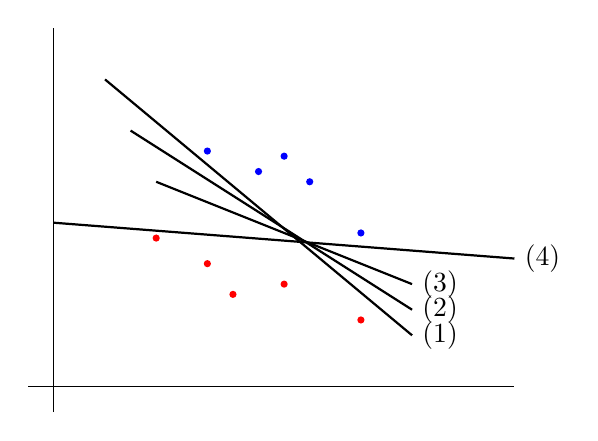
\begin{tikzpicture}[scale=0.65]
          % Draw axes
          \draw[-] (-0.5,0) -- (9,0);
          \draw[-] (0,-0.5) -- (0,7);
          
          % Intersection point
          \coordinate (I) at (4,3);
          
          % Draw numbered lines
          \draw[thick] (1,6) -- (7,1) node[right] {(1)};
          \draw[thick] (1.5,5) -- (7,1.5) node[right] {(2)};
          \draw[thick] (2,4) -- (7,2) node[right] {(3)};
          \draw[thick] (0,3.2) -- (9,2.5) node[right] {(4)};
          
          % Add blue points (above lines)
          \fill[blue] (3,4.6) circle (2pt);
          \fill[blue] (4,4.2) circle (2pt);
          \fill[blue] (5,4) circle (2pt);
          \fill[blue] (6,3) circle (2pt);
          \fill[blue] (4.5,4.5) circle (2pt);
          
          % Add red points (below lines)
          \fill[red] (2,2.9) circle (2pt);
          \fill[red] (3,2.4) circle (2pt);
          \fill[red] (3.5,1.8) circle (2pt);
          \fill[red] (4.5,2) circle (2pt);
          \fill[red] (6,1.3) circle (2pt);
        \end{tikzpicture}
        \caption{Planes such as (1) and (4) are ``too close" to the positive and negative samples. } 
        \label{fig:svm_intro_1}
      \end{subfigure}
      \hfill
      \begin{subfigure}[b]{0.45\textwidth} 
        \centering 
        \begin{tikzpicture}[scale=0.65]
          % Draw axes
          \draw[-] (-0.5,0) -- (9,0);
          \draw[-] (0,-0.5) -- (0,7);
          
          % Intersection point
          \coordinate (I) at (4,3);
          
          % Draw numbered lines
          \draw[thick] (1,5) -- (7,1.5);
          \draw[dotted, thick] (1,5.8) -- (7,2.3);
          \draw[dotted, thick] (1,4.2) -- (7,0.7);
          
          % Add blue points (above lines)
          \fill[blue] (3,4.6) circle (2pt);
          \fill[blue] (4,4.2) circle (2pt);
          \fill[blue] (5,4) circle (2pt);
          \fill[blue] (6,3) circle (2pt);
          \fill[blue] (4.5,4.5) circle (2pt);
          
          % Add red points (below lines)
          \fill[red] (2,2.9) circle (2pt);
          \fill[red] (3,2.4) circle (2pt);
          \fill[red] (3.5,1.8) circle (2pt);
          \fill[red] (4.5,2) circle (2pt);
          \fill[red] (6,1.3) circle (2pt);
        \end{tikzpicture}
        \caption{SVMs try to find the separating hyperplane with the best minimum margin.} 
        \label{fig:svm_intro2}
      \end{subfigure} 
      \caption{Motivating problem} 
      \label{fig:svm_intro} 
    \end{figure}
  \end{example} 

  We want to formalize the concepts of these margins that we wish to maximize. Furthermore, this problem is not well defined since we can just set $w$ to be $0$ or an arbitrarily high norm vector, which makes this problem ill-posed. Therefore, we will need some constraints as well. 

\subsection{Functional and Geometric Margins} 
  
  To do this, we will define two terms. 

  \begin{definition}[Geometric margin]
    Given a point $\mathbf{x}_0$ and a hyperplane of equation $\mathbf{w} \cdot \mathbf{x} + b = 0$, the distance from $\mathbf{x}_0$ to the hyperplane, known as the \textbf{geometric margin}, can be computed with the formula 

    \begin{equation}
      d = \frac{|\mathbf{x}_0 \cdot \mathbf{w} + b|}{||\mathbf{w}||}  
    \end{equation} 

    Therefore, the geometric margin of the $i$th sample with respect to the hypothesis $f$ is defined 

    \begin{equation}
      \gamma_i = \frac{y_i \, (\mathbf{w} \cdot \mathbf{x}_i + b)}{||\mathbf{w}||} 
    \end{equation} 
  \end{definition}

  We wish to optimize the parameters $\mathbf{w}, b$ in order to maximize the minimum of the geometric margins (the distance between the closest point and the hyperplane). 

  \begin{equation}
    \argmax_{\mathbf{w}, b} \min_i \gamma_i = \argmax_{\mathbf{w}, b} \bigg\{ \frac{1}{||\mathbf{w}||} \min_i \big[y_i \, (\mathbf{w} \cdot \mathbf{x}_i + b) \big] \bigg\}
  \end{equation}

  Direct solution of this optimization problem would be very complex, and so we convert this into an equivalent problem that is much easier to solve. Note that the solution to the above term is not unique. If there was a solution $(\mathbf{w}^\ast, b^\ast)$, then 

  \begin{equation}
    \frac{y_i (\mathbf{w} \cdot \mathbf{x}_i + b)}{||\mathbf{w}||} = \frac{y_i (\lambda \mathbf{w} \cdot \mathbf{x}_i + \lambda b)}{||\lambda \mathbf{w}||}  
  \end{equation}

  That is, the geometric margin is not sensitive to scaling of the parameters of the hyperplane. Therefore, we can scale the numerator and the denominator by whatever we want and use this freedom to set 

  \begin{equation*}
    y_i ( \mathbf{w} \cdot \mathbf{x}_i + b ) = 1 
  \end{equation*}
  
  for the point that is closest to the surface. In that case, all data points will satisfy the constraints 

  \begin{equation*}
    y_n (\mathbf{w} \cdot \mathbf{x}_i + b) \geq 1
  \end{equation*}

  In the case of data points for which the equality holds, the constraints are said to be \textit{active}, whereas for the remainder they are \textit{inactive}. Therefore, it will always be the case that $\min_i \big[ y_i \, (\mathbf{w} \cdot \mathbf{x}_i + b)\big] = 1$, and the constraint problem reduces to 

  \begin{equation}
    \argmax_{\mathbf{w}, b} \frac{1}{||\mathbf{w}||} = \argmin_{\mathbf{w}, b} \frac{1}{2} ||\mathbf{w}||^2 \text{ subject to constraints } y_i (\mathbf{w} \cdot \mathbf{x}_i + b) \geq 1 
  \end{equation}

  This final step is the most significant step in this derivation and may be hard to wrap around the first time. So we dedicate the next subsubsection for this. 

  
  We could just work straight with this geometric margin, but for now, let's try to extend what we did with the perceptron into SVMs. We will find out that extending the concept of functional margins into SVMs leads to ill-defined problems. In the perceptron, we wanted to construct a function $f(\mathbf{x}) = \mathbf{w} \cdot \mathbf{x} + b$ such that 
  \begin{equation*}
    y_i \, f(\mathbf{x}_i) \geq 0 \text{ for all } i = 1, 2, \ldots, N
  \end{equation*}

  \begin{definition}[Functional Margin]
    The value of $y_i \, f(\mathbf{x}_i)$ gives us our confidence on our classification, and in a way it represents a kind of distance away from the separating hyperplane (if this value was $0$, then we would be 50 50 split on whether to label it positive or negative). Therefore, we shall define 
    \begin{equation*}
        \hat{\gamma}_i = y_i f(\mathbf{x}_i) 
    \end{equation*}
  as the \textbf{functional margin} of $(\mathbf{w}, b)$ with respect to the training sample $(\mathbf{x}_i, y_i)$. Therefore, the smallest of the function margins can be written 
  \begin{equation*}
      \hat{\gamma} = \min_i \gamma_i 
  \end{equation*}
  called the \textbf{function margin}. 
  \end{definition}

  Note that the geometric margin and functional margin are related by a constant scaling factor. Given a sample $(\mathbf{x}_i, y_i)$, we have 
  \begin{equation*}
      \mathrm{Geometric Margin} = \frac{y_i \, (\mathbf{w} \cdot \mathbf{x}_i + b)}{||\mathbf{w}||_2} = \frac{\mathrm{Functional Margin}}{||\mathbf{w}||_2}
  \end{equation*}

  As we can see, the perceptron works with the functional margin, and since it does not care about how large the margin is (just whether it's positive or negative), we are left with an underdetermined system in which there exists infinite $(\mathbf{w}, b)$'s. Now what we want to do is impose a certain minimum margin $\gamma > 0$ and solve for $(\mathbf{w}, b)$ again, and keep increasing this $\gamma$ until there is some unique solution. We can view this problem in two ways: 
  \begin{enumerate} 
      \item Take a specific minimum margin $\gamma$ and find a $(\mathbf{w}, b)$, which may not exist, be unique, or exist infinitely that satisfies 
          \begin{equation*}
              y_i f(\mathbf{x}) = y_i ( \mathbf{w} \cdot \mathbf{x} + b) \geq \gamma \text{ for all } i = 1, \ldots, N 
          \end{equation*}
      \item Take a specific $(\mathbf{w}, b)$ and calculate the maximum $\gamma$ that satisfies the constraint equations above.  
  \end{enumerate}

  They're both equivalent problems, but both ill-posed if we look at (2). Since the samples are linearly separable by assumption, we can say that there exists some $\epsilon > 0$ such that $y_i f(\mathbf{x}_i) \geq \epsilon$ for all $i$. Therefore, if we just scale $(\mathbf{w}, b) \mapsto (\lambda \mathbf{w}, \lambda b)$ for some large $\lambda$, this leads to the solution for $\gamma$ being unbounded. We can see in Figure $\ref{fig:scaling_problem}$ that we can increased confidence at no cost. Looking at (1), we can also see that if $(\mathbf{w}, b)$ does exist, then every other $(\lambda \mathbf{w}, \lambda b)$ for $\lambda > 1$ satisfies the property.   

  \begin{figure}[H] 
    \centering 
    \begin{subfigure}[b]{0.32\textwidth} 
      \centering 
      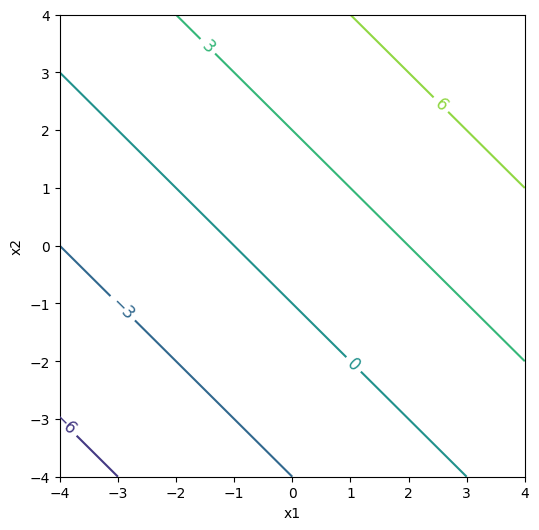
\includegraphics[width=\textwidth]{img/scaling1.png} 
      \caption{$f(x) = x_1 + x_2 + 1$} 
      \label{fig:original_scaled}
    \end{subfigure} 
    \hfill    
    \begin{subfigure}[b]{0.32\textwidth} 
      \centering 
      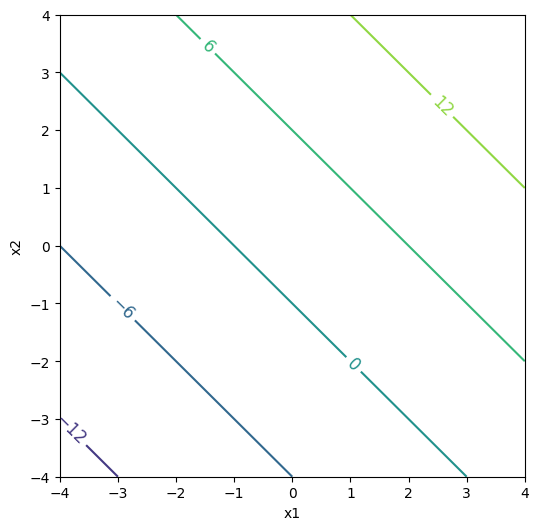
\includegraphics[width=\textwidth]{img/scaling2.png} 
      \caption{$f(x) = 2 x_1 + 2 x_2 + 2$} 
      \label{fig:two_times_scaled}
    \end{subfigure} 
    \hfill
    \begin{subfigure}[b]{0.32\textwidth} 
      \centering 
      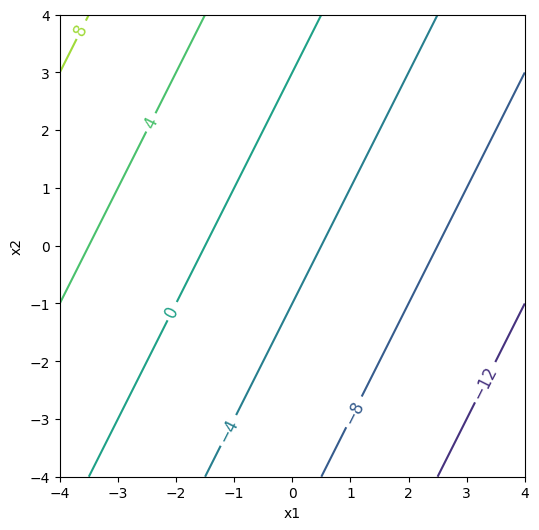
\includegraphics[width=\textwidth]{img/scaling3.png} 
      \caption{$f(x) = -2x_1 + x_2 - 3$} 
      \label{fig:something_else}
    \end{subfigure} 
    \caption{From (a), you can see that simply multiplying everything by two automatically increases our confidence by $2$, meaning that the functional margin can be scaled arbitrarily by scaing $(\mathbf{w}, b)$. There are still too many degrees of freedom in here and so extra constraints must be imposed. } 
    \label{fig:scaling_problem} 
  \end{figure}

\subsection{Analytical Solution} 

  To minimize the equations with the constraint equations, we can use the method of Lagrange multipliers, which leads to to Lagrangian 
  \[\mathcal{L}(\mathbf{w}, b, \boldsymbol{\alpha}) = \frac{1}{2} ||\mathbf{w}||^2 - \sum_i \alpha_i \big[ y_i (\mathbf{w} \cdot \mathbf{x}_i + b) - 1\big]\]
  We can take the gradients with respect to $\mathbf{w}$ and $b$ and set them to $0$, which gives the two conditions 
  \begin{align*} 
    \mathbf{w} & = \sum_i \alpha_i y_i \mathbf{x}_i \\
    0 & = \sum_i \alpha_i y_i \mathbf{x}_i 
  \end{align*}

  Now let's substitute our evaluated $\mathbf{w}$ back into $\mathcal{L}$, which gives the \textbf{dual representation} of the maximum margin problem in which we maximize  
  \begin{align*} 
      L & = \frac{1}{2} \bigg( \sum_i \alpha_i y_i \mathbf{x}_i \bigg) \bigg( \sum_j \alpha_j y_j \mathbf{x}_j \bigg) - \sum_{i} \alpha_i y_i x_i \cdot \bigg[ \sum_j \alpha_j y_j x_j \bigg] - \sum_i \alpha_i y_i b + \sum_i \alpha_i \\ 
        & = \sum_i \alpha_i - \frac{1}{2} \sum_{i, j} \alpha_i \alpha_j y_i y_j \, \mathbf{x}_i \cdot \mathbf{x}_j 
  \end{align*}
  The summation with the $b$ in it is $0$ since we can pull the $b$ out and the remaining sum is $0$ from before. Now the optimization only depends on the dot product $\mathbf{x}_i \cdot \mathbf{x}_j$ of all pairs of sample vectors, which is very interesting. We will see more of this when we talk about kernel methods. Now, we need to solve the dual problem 
  \[\max_{\boldsymbol{\alpha}} \mathcal{L}(\boldsymbol{\alpha})\]
  which can be done using some generic quadratic programming solver or some other method to get the optimum $\boldsymbol{\alpha}^\ast$, which gives us 
  \[\mathbf{w}^\ast = \sum_i \alpha_i^\ast y_i \mathbf{x}_i\]

\subsection{Significance Tests and Confidence Sets}

\subsection{Concentration Bounds} 

\subsection{Nonseparable Case} 


\section{Gaussian/Linear Discriminant Analysis}

\subsection{Discriminative vs. Generative Models}

  Now we introduce our first example of a generative model, which introduces another division between models (in addition to parametric vs nonparametric, frequentist vs bayesian). Generally, there are two ways to model $\mathbb{P}_{Y \mid X = x}$. 

  \begin{definition}[Discriminative Models]
    \textbf{Discriminative models} attempt to do this directly by  modeling only the conditional probability distribution $\mathbb{P}_{Y \mid X = x}$. We don't care about the underlying distribution of $X$, but rather we just want to try and predict $Y$ given $X$. Essentially, we are trying to approximate the conditional expectation $h(X) = \mathbb{E}[Y \mid X]$, which is the best we can do. Given $X = x$, we use our model of $\mathbb{P}_{Y \mid X = x}$, and our hypothesis function will predict the its mean. 
    \begin{equation}
      h(x) = \mathbb{E}[Y \mid X = x]
    \end{equation}
  \end{definition}

  \begin{definition}[Generative Models]
    \textbf{Generative models} approximate this conditional probability by taking a more general approach. They attempt to model the joint probability distribution $\mathbb{P}_{X \times Y}$ (also called \textbf{inference}), which essentially gives everything we need about the data. Doing this allows us to \textit{generate} more data (hence the name), which may be useful. 
        
    One way to approximate the joint distribution is to model the conditional distribution $\mathbb{P}_{X \mid Y = y}$, which gives the distribution of each labels. Now combined with the probability measure $\mathbb{P}_Y$, we can get the joint distribution. Usually in classification, the $\mathbb{P}_Y$ is easy to approximate (the MLE is simply the fequencies of the labels), so conventionally, modeling $\mathbb{P}_{X \times Y}$ and modeling $\mathbb{P}_{X \mid Y = y}$ are considered the same thing. Once we have these, we can calculate the joint distribution, but in high-dimensional spaces this tends to be computationally hard. Therefore, we usually resort to simply calculating $\mathbb{P}_{X \mid Y = y}$ and then using Bayes rule to approximate 
    \begin{equation}
      \mathbb{P}_{Y \mid X} = \frac{\mathbb{P}_{X \mid Y} \mathbb{P}_Y}{\mathbb{P}_X}
    \end{equation}
    where the normalizing term is computed using Monte Carlo simulations. 
  \end{definition}

  This is the first example of a generative model. In GDA, we basically write the likelihood as 
  \begin{equation}
    \prod_{i=1}^n p(x_i, y_i) = \prod_{i} p(x_i \mid y_i) p(y_i)
  \end{equation}
  where each $p(x_i \mid y_i)$ is Gaussian and $p(y_i)$ is Bernoulli. This specifies $p(x_i, y_i)$ and therefore is called a generative model. In logistic regression, we have 
  \begin{equation}
    \prod_{i=1} p(x_i, y_i) = \bigg( \prod_i p(y_i \mid x_i) \bigg) \bigg( \prod_i p(x_i) \bigg)
  \end{equation}
  and the first term is the logistic function and the second term is unknown. We only use the first part to classify, and this is a discriminative model. You can be agnostic about the data generating process and you can work with less data since there are less things to fit. Some people ask why should you model more unless you have to, so people tend to try to model the minimum, which is why logistic regression is more popular. 

\subsection{Construction}

  GDA assumes that $\mathbb{P}(x\,|y)$ is distributed according to a multivariate Gaussian distribution. Let us assume that the input space is $d$-dimensional and this is a binary classification problem. We set 
  \begin{align*} 
    y & \sim \text{Bernoulli}(\pi) \\
    x\,|\,y = 0 & \sim \mathcal{N}_d (\mu_0, \Sigma) \\
    x\,|\,y = 1 & \sim \mathcal{N}_d (\mu_1, \Sigma)
  \end{align*}
  This method is usually applied using only one covariance matrix $\Sigma$. The distributions are
  \begin{align*}
    p(y) & = \pi^y (1 - \pi)^{1-y} \\
    p(x\,|\,y = 0) & = \frac{1}{(2\pi)^{d/2} |\Sigma|^{1/2}} \exp \bigg(-\frac{1}{2} (x - \mu_0)^T \Sigma^{-1} (x - \mu_0)\bigg) \\
    p(x\,|\,y= 1) & = \frac{1}{(2\pi)^{d/2} |\Sigma|^{1/2}} \exp \bigg(-\frac{1}{2} (x - \mu_1)^T \Sigma^{-1} (x - \mu_1)\bigg)
  \end{align*}
  Now, what we have to do is optimize the distribution parameters $\pi \in (0, 1) \mathbb{R}, \mu_0 \in \mathbb{R}^d, \mu_1 \in \mathbb{R}^d, \Sigma \in \text{Mat}(d \times d, \mathbb{R}) \simeq \mathbb{R}^{d \times d}$ so that we get the best-fit model. Assuming that each sample has been picked independently, this is equal to maximizing 
  \begin{equation}
    L(\pi, \mu_0, \mu_1, \Sigma) = \prod_{i=1}^n \mathbb{P}\big( x^{(i)}, y^{(i)}\,;\, \pi, \mu_0, \mu_1, \Sigma\big)
  \end{equation}
  which is really just the probability that we get precisely all these training samples $(x^{(i)}, y^{(i)})$ given the 4 parameters. This can be done by optimizing its log-likelihood, which is given by 
  \begin{align*}
    l(\pi, \mu_0, \mu_1, \Sigma) & = \log \prod_{i=1}^n \mathbb{P}(x^{(i)}, y^{(i)}; \pi, \mu_0, \mu_1, \Sigma) \\
    & = \log \prod_{i=1}^n \mathbb{P}( x^{(i)} \,|\, y^{(i)}; \mu_0, \mu_1, \Sigma) \, \mathbb{P}(y^{(i)}; \pi) \\
    & = \sum_{i=1}^n \log \bigg( \mathbb{P}( x^{(i)} \,|\, y^{(i)}; \mu_0, \mu_1, \Sigma) \, \mathbb{P}(y^{(i)}; \pi) \bigg)
  \end{align*}
  and therefore gives the maximum likelihood estimate to be 
  \begin{align*}
    \pi & = \frac{1}{N} \sum_{n=1}^N 1\{y^{(n)} = 1\} \\
    \boldsymbol{\mu}_0 & = \frac{\sum_{n=1}^n 1_{\{y^{(n)} = 0 \}} \mathbf{x}^{(n)}}{\sum_{n=1}^N 1_{\{y^{(n)} = 0 \}}} \\
    \boldsymbol{\mu}_1 & = \frac{\sum_{n=1}^n 1_{\{y^{(n)} = 1\}} \mathbf{x}^{(n)}}{\sum_{n=1}^N 1_{\{y^{(n)} = 1 \}}} \\
    \boldsymbol{\Sigma} & = \frac{1}{N} \sum_{n=1}^N (\mathbf{x}^{(n)} - \mu_{y^{(n)}}) (\mathbf{x}^{(n)} - \mu_{Y^{(i)}})^T 
  \end{align*}

  A visual of the algorithm is below, with contours of the two Gaussian distributions, along with the straight line giving the decision boundary at which $\mathbb{P}(y=1\,|\,x) = 0.5$. 
  \begin{figure}[H]
      \centering
      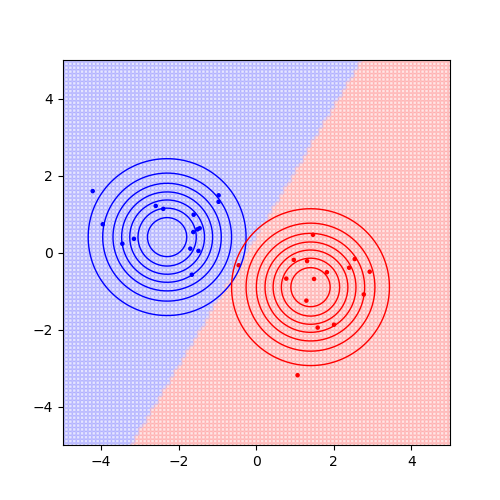
\includegraphics[scale=0.7]{img/GDA.png}
      \caption{GDA of Data Generated from 2 Gaussisans centered at $(-2.3, 0.4)$ and $(1.4, -0.9)$ with unit covariance. The decision boundary is slightly off since MLE approximates the true means. }
      \label{fig:gda}
  \end{figure}



\bibliography{./bibfile}
\bibliographystyle{alpha}
\end{document}
